\chapter{Discussion}
\label{ch:discussion}

\section{Volume Registration}

The comparison of the simulated and clinical brain rs-fMRIs using the local and global motion metrics showed different effects for each data set.

In the simulated images, there was a decrease in both the FD and DVARS values for both registration types. The change in the distribution of FD for both registration types was statistically significant for 40 sequences at $p < 0.05$. However, the difference in the DVARS distributions was only significant at $p < 0.05$ for three sequences. The global metrics had statistically significant differences in the Dice and MI distributions for all three sequence types (original, traditionally registered, and DAG-registered), with the DAG-registered sequences having the overall highest values and smallest distributions.

For the preadolescent images, the distributions of the local motion metrics of the traditionally registered sequences were more similar to those of the original sequences than the distributions of the DAG-registered sequences. The DAG-based registration actually saw an increase in the local motion metrics. Specifically, there was a large spike in the mean and standard deviation of the DVARS values in the first 50 image volumes of the sequences. The magnitude and duration of this increase suggests that there may be a factor severely impacting a large number of preadolescent sequences in the first half of the scan. It is possible that many preadolescent subjects exhibited similar motion patterns in this part of the scan that were difficult for the DAG-based registration to correct.

The neonatal images experienced a different effect from both registrations. The FD distributions remained relatively consistent while the mean and standard deviations of the DVARS distributions increased for both registration types. These distribution changes were not expected: while registration is not designed to address the signal-related effects of motion, it was not expected to exacerbate them. As this type of change was specific to the neonatal images, it is possible that there are tissue properties specific to neonatal brains that caused these changes.

The registrations had the opposite effects on the fetal brain images than they did on the preadolescent images. The distributions for the local motion of the DAG-registered sequences were more similar to those of the original sequences than the traditionally registered distributions were. Additionally, there were several spikes in the FD of the traditionally registered sequences that were not present in the FD for the DAG-registered sequences. When comparing the numbers of usable image volumes from each sequence type, the number of image volumes meeting the FD threshold was consistent between all three sequence types. The original and DAG-based sequences had the same number of image volumes meeting the DAVRS thresholds, though the traditional registration had an increased number of volumes meeting that threshold. These results suggest that the DAG-based registration framework may be more effective at reducing the effects of motion (or at least not exacerbating them) than the traditional framework.

For all the clinical brain images, there was a decrease in the number of usable image volumes after registration. While this decrease may suggest that volume registration degrades an image, it does not mean that volume registration should be removed from the retrospective motion correction toolkit. Before registration, the relationships between the position of the patient at every time point are unknown. Registration is similar to looking in Schrodinger's box: until we do, we cannot quantify the effects of patient motion on the acquired sequence.

The changes in the similarity matrix value distributions were comparable overall for the clinical images.

In the set of placenta images, both registration types increased the mean and standard deviations of the distributions of both local motion metrics. However, even with these changes, both registration types improved the number of image volumes meeting the DVARS threshold. This result was completely unique to the placenta images and is likely related to the difference between the tissue properties of the brain and the placenta.

An additional analysis was performed for the simulated images. The goal of this analysis was to evaluate the effects of volume registration on the brain signal present in an rs-fMRI image. It was found that the DAG-registered sequences had correct voxel classifications when compared to the DMN ROI than the traditional registration did. 

This finding has exciting potential. Subject motion during rs-MRI scans affects both the recorded position and orientation of the subject as well as the established magnetic spin gradients within the skull and the susceptibility recorded in each voxel. The primary focus of volume registration has been to reduce the positional effects of motion. Correction of the spin history effects and the susceptibility effects are considered to be a separate albeit related area of research. The results of the independent component analysis of the simulated images suggest that the DAG-based registration may contribute to the reduction of the signal-based effects of motion. It could potentially be coupled with prospective motion monitoring techniques, $B_0$ field maps, and navigator sequences to address the other half of the motion problem.

\section{Characterizing Motion}

In addition to the evaluation of motion within the images, clustering techniques were used to identify groups of subjects with similar motion patterns in their original sequences. Agglomerative clustering was used to confirm the existence of similar motion patterns between patients. The agglomerative clustering results consisting of a heatmap and a dendrogram were combined with two sets of labels: the disease status and age group of each subject. Examination of the dendrograms and heatmaps coupled with the labels suggested that subjects in the same age group were more likely to exhibit similar motion patterns to each other than to subjects in other age groups. To reinforce this theory, k-means clustering and spectral clustering were also performed on the data. The labels produced by the clustering techniques were compared to the age group labels. The composition of the clusters reinforces the theory that patient motion patterns vary more between age groups than among age groups.

Additional analyses could be performed to evaluate the computer-detectable differences in patient groups in more detail. The models presented in the previous chapter were generated with each using a single metric type. Each metric only measures one property of the image volumes. It is possible that combinations of metrics measuring different properties could be used to better separate patient groups. For example, the combination of the FD values and the DVARS values could more comprehensively categorize subjects based on the effects of motion, BOLD signal change, and background noise.

\section{Expectations vs. Outcomes}

In Chapter \ref{ch:data}, we outlined the expected differences in motion patterns between the clinical groups, the expected effects of the registration technique on data from each clinical group, and the expected groups that could be identified via clustering.

We predicted that the neonatal subjects would demonstrate the least motion and the fetal subjects would demonstrate the most motion out of the clinical cohorts. Comparing the FD and DVARS of the original image sequences confirms that the neonatal subjects demonstrated the least motion, but the comparison between the preadolescent and fetal subject motion is slightly more complicated. Figure \ref{fig:orig-local-motion} shows a direct comparison between the average local motion metrics for the original sequences. It is only in comparing both the FD and DVARS that we can see that the fetal subjects do move more than the preadolescent subjects.

\begin{figure}
	\centering
	\begin{subfigure}{0.4\textwidth}
		\centering
		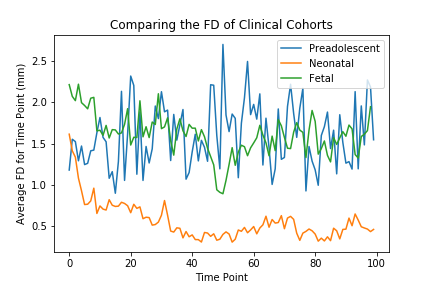
\includegraphics[width=1.0\textwidth]{7/figures/orig-avg-fd.png}
		\caption{Average FD of Original Sequences.}
	\end{subfigure}
	\hspace{0.05\textwidth}
	\begin{subfigure}{0.4\textwidth}
		\centering
		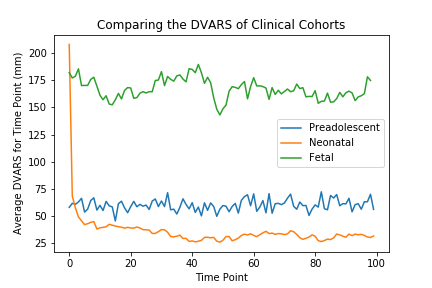
\includegraphics[width=1.0\textwidth]{7/figures/orig-avg-dvars.png}
		\caption{Average DVARS of Original Sequences.}
	\end{subfigure}
	
\caption{The average local motion metrics for all original sequences show that the neonatal subjects move the least, though differences between fetal and preadolescent motion is more clear in (b).}
\label{fig:orig-local-motion}
\end{figure}

Due to the physical constraints on subjects from each population during the scan, we expected the registration frameworks to have different effects on the clinical cohorts. We expected that the DAG-based registration would have the best performance on the fetal subjects, but it was difficult to develop more granular hypotheses about each framework's effects on each clinical group. In general, we saw a comparable performance between the registration types for the neonatal cohort. The DAG-based framework was less effective at reducing motion in the preadolescent cohort than the traditional framework was. We also saw the DAG-based registration preserve the local motion in the fetal images while the traditional registration increased local motion.  Out of these three sets of effects, the DAG-registration did indeed perform best on the fetal cohort. 

Finally, we expected to see different patterns of motion dependent on clinical and age groups. In our clustering analysis of the population-wide motion patterns, we did not see distinct groups of healthy and CHD subjects based on their motion parameters. We did, however, see a relationship between age group and motion metrics. These results do not mean that there are no relationships between CHD disease status and motion: rather, they suggest that disease and motion relationships may occur on an age-group level rather than a lifespan level.

\section{Relation to Existing Work}

\subsection{MRI Simulations} 

The idea of simulated MRIs originated in the 1980s. Bobman et al. suggested a process of MR image synthesis, then demonstrated its validity by creating synthetic spin-echo brain MRIs and comparing the simulated images to clinical images \cite{Bobman1985}. Since then, several MRI simulation software tools have been developed. Herein, we discuss two of these tools and compare them to our simulation tool.

The FMRIB group developed a simulation tool called \href{https://fsl.fmrib.ox.ac.uk/fsl/fslwiki/POSSUM}{POSSUM} (Physics-Oriented Simulated Scanner for Understanding MRI) \cite{Drobnjak2006} \cite{Drobnjak2010}. POSSUM offers a realistic, physics-based simulation of structural, functional, and diffusion tensor images. It requires a gradient echo pulse sequence and a segmented object with known tissue properties as inputs for the simulation. It allows the user a high degree of control over the physical properties to be simulated. The user can specify the pulse sequence information, the method for generating brain signal, the addition of motion and noise, and the method for image reconstruction. Both a GUI and a command-line interface are available for POSSUM. 

The biggest drawback to POSSUM is the degree of MR physics knowledge needed to use it effectively. For MR physicists, specifying the details of a pulse sequence may be trivial. For researchers from other fields, customizing pulse sequence parameters, an example of which can be seen in Figure \ref{fig:possum}, can be a challenging task. These customizations may even be unnecessary depending on the goals a researcher hopes to achieve using the simulated data.

\begin{figure}
\centering
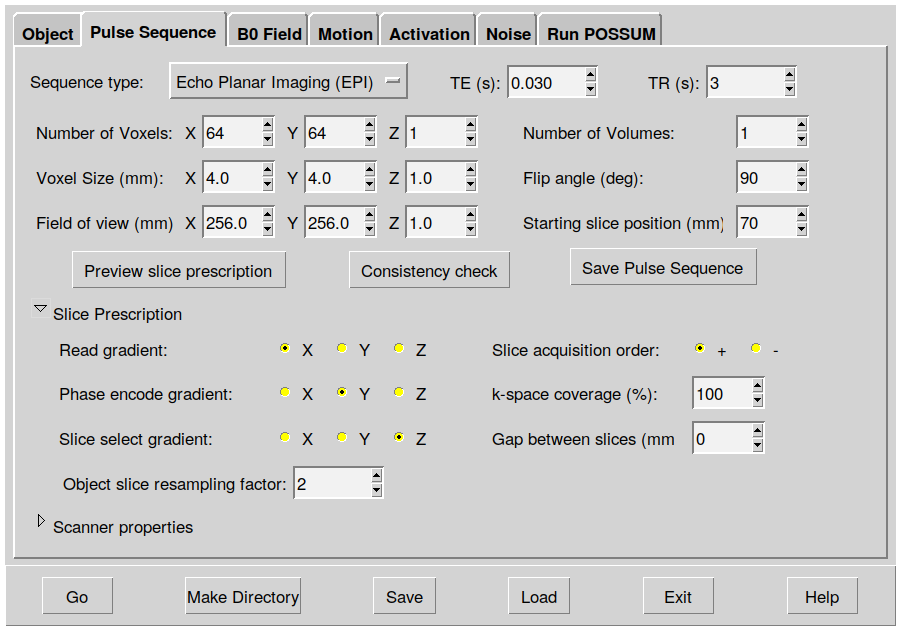
\includegraphics[width=.6\textwidth]{7/possum-gui.png}
\caption{The ``Pulse Sequence'' specifications page in the POSSUM GUI}
\label{fig:possum}
\end{figure}


If a researcher's goal is to test the impact of a new MRI processing technique on known signals in an image, the BrainWeb MRI simulator might be a better option than POSSUM. BrainWeb was created and is actively developed by the \href{mcgill.ca/bic/}{McConnell Brain Imaging Centre} at McGill University to assist in validation computer-aided MRI analysis tools \cite{kwan1999mri} \cite{collins1998design} \cite{cocosco1997brainweb} \cite{kwan1996extensible}. A set of simulated images have been generated using BrainWeb and can be found in the BrainWeb Simulated Brain Database (SBD). The SBD contains simulated images for healthy subjects and for subjects who have lesions due to multiple sclerosis.

Custom simulations can be generated on the BrainWeb server by submitting a request via a browser. The simulation request form has three areas that can be customized: the type of brain to simulate, the MR pulse sequence, and the imaging artifacts. The simulation is run on the server and the user is notified via email when the simulated images are ready to download. 

BrainWeb's simulator is slightly more approachable than POSSUM: a limited number of pulse sequence parameters are available to customize, and a description is listed next to each parameter in the pulse sequence and imaging artifacts sections. However, the user has slightly less control over the simulated image. The brain models used by BrainWeb are healthy brains or brains with MS lesions. It is not an option for the user to upload an image to use as the structural information in the sequence. For our purposes, the most significant limitation of BrainWeb is that it only simulates structural images. 

Our simulation tool, SPECTr, is one of the few tools which simulates resting-state fMRIs. It offers the opportunity for researchers to explore the effects of their motion correction techniques on the BOLD signal, background noise, and patient motion using a lightweight simulation that can be run on a personal computer. It should be noted that SPECTr is not a substitute for the physics-based models in POSSUM and BrainWeb: it is intended to evaluate signal changes in rs-fMRI sequences as a result of post-acquisition image processing.

\subsection{Volume Registration} 

To the best of our knowledge, the only other study that has used a variant of the DAG-based method was performed by Liao et al. \cite{Liao2016}. Liao et al’s dataset consisted of 10 fetal rs-fMRIs. In each of these sequences, the fetal brain, fetal liver, and placenta were manually segmented in the first volume of the sequence as well as in five other randomly chosen volumes. These overlap of these manual segmentations before and after registration, as measured using the Dice coefficient, was used to quantify the amount of motion in each sequence. Even though the Dice coefficients increase more in each sequence after Liao et al.’s registration than after traditional registration, their measure of positional change fails to quantify any changes in position between any other pairs of volumes that do not have manual segmentations. 

The fetal images used in Liao et al.'s study included images of singleton, twin, and triplet pregnancies. There is significant potential value in the study of fetal motion in multifetal pregnancies. Considering the motion patterns alone, it would be expected that the singleton pregnancies have different motion patterns than the multifetal pregnancies.

\subsection{Age Group Specific Motion}

It has been established that motion is often correlated with patient age in the adolescent population. Satterthwaite et al. specifically designed an imaging study of adolescents ages 8-23 such that patient age and motion were uncorrelated \cite{Satterthwaite2012} % ELEPHANTS check citation
In our study, patient age was described only as fetal, neonatal, or preadolescent despite a range of ages in each group. We establish that there are characteristics of patient motion specific to each group, but we did not consider more granular ranges of patient age. Additional analyses would need to be considered to determine whether the post-conceptual age for fetal and neonatal subjects impacts motion characteristics. 

In the fetal cohort, there may be motion characteristics linked to post-conceptual age. As a fetus grows, the amount of room in the uterus in which it can move decreases. However, as the fetal brain develops, the fetus may begin to move in different ways to test its biological systems. 

Studies involving neonatal cohorts often track two ages for the subjects: the post-conceptual age and the age since birth. The relationship between these two ages and a neonate's brain development could impact the amount of motion exhibited during a scan.

\section{Limitations}

\subsection{Spin History and Susceptibility Effects of Motion}

As discussed in Chapter \ref{ch:mri}, patient motion has three effects on the acquired images. In this work, we have provided an analysis of how one step of retrospective motion correction can be used to reduce the positional effects of motion. While some of the clinical images also saw changes in the signal-related effects of motion (spin history effects and susceptibility effects), registration is not designed to alleviate these effects of motion. Comprehensive motion correction pipelines can be used to filter and denoise sequences registered using the DAG-based framework. Furthermore, additional scan types such as $B_0$ field maps or navigator sequences contain valuable information that can be used to correct the spin history and susceptibility effects of motion directly.

\subsection{Runtime}

One topic we have not yet addressed in this work is the amount of time needed to perform the registrations and motion measurements. Herein, we compare the amount of time needed to run each registration framework. Assuming each operation for the same initial sequence is performed on the same computing hardware, the operations are limited by the number of image volumes in the rs-fMRI, $N$. We define $r$ as the maximum amount of time to perform one pairwise volume registration.

In traditional registration, the contents of a 4D image sequence containing $N$ image volumes are all aligned to the contents of a single image volume. At face value, the runtime $R$ of the registration is $r*N$. However, there are no dependencies of the registration of one volume in the registration of another volume. Therefore, all registrations can theoretically be performed at the same time in parallel. Parallelizing the registrations for a single sequence means that the expected runtime of the sequence registration should decrease to 

\begin{equation}
R_{trad} = \frac{hrN}{p}
\end{equation} 

\noindent where $h$ is a factor specific to the hardware properties of the computer being used and $p$ is the degree to which the registration can be parallelized. In a scenario where the computer has enough power and resources to run all $N$ pairwise volume registrations in parallel, the runtime decreases to $hr$. 

This decrease due to parallelization is only an option for the traditional registration framework. For the DAG-based registration framework, each pairwise volume registration is dependent on the affine transformation produced by the previous volume's registration. While this dependency accounts for the important temporal relationships between subsequent image volumes, it means that the image volume registrations must be performed in series, not in parallel. As a result, the runtime for the DAG-based registration is

\begin{equation}
R_{dag} = hrN.
\end{equation}

\begin{table}
\centering
\caption{The statistics for the runtimes of the registrations of 17 healthy neonatal subjects demonstrate that runtime of registration is not a trivial concern.}
\label{tab:runtime-example}
\begin{tabular}{|l|c|c|}
\hline
\textbf{Registration Framework} & \textbf{Traditional} & \textbf{DAG-based} \\ \hline
\textit{Average (HH:MM:SS)}     & 00:41:55.25          & 01:38:20.02        \\ \hline
\textit{Median (HH:MM:SS)}      & 00:44:44.20          & 01:38:42.63        \\ \hline
\textit{Maximum (HH:MM:SS)}     & 01:21:46.95          & 03:02:36.10        \\ \hline
\end{tabular}
\vspace{0.05\textwidth}
\end{table}

An example of the power of parallelization can be seen in Table \ref{tab:runtime-example}. This table shows the average, median, and maximum runtimes for both registration types for a subset of high-motion sequences belonging to healthy neonatal subjects on a desktop computer with 8 cores. Each of the runtime statistics for the DAG-based registration is almost twice as much as the corresponding runtime statistic for the traditional registration.

There are at least two occasions where the runtime of the registration frameworks may suggest the use of the traditional registration over the DAG-based registration. The first occasion is when the registered image is needed urgently. The second is when there are many registrations to perform. Access to computational clusters may help decrease the registration time, but this decrease could be expected for both frameworks.

\subsection{Manual Segmentations}

All images used in these analyses consisted of brain tissue against an empty background. The images had undergone processing to remove tissues outside the skull, either using automated tools or manual segmentation. The use of manual segmentation with multiple annotators has the potential to confound the results of motion correction experiments. The segmentation process may not remove all non-brain tissue from the image. Those images would then contain brain tissue, non-brain tissue, and dark background. 

The combination of these three tissue types has the potential to cause problems during the registration of the manually segmented images. The registration process optimizes the alignment of values in a pair of images. In some cases, the registration reaches a state where the lowest-cost alignment aligns anything not part of the background together, not specifically brain tissue to brain tissue. While these alignments do have the lowest cost, the results are not physically correct. This problem is difficult to detect in the metrics extracted from the image sequences: the metrics only measure the properties of the voxel values in the sequence, not of the physiological information it contains. 

Specifically, this limitation pertains to our fetal scans. The masks generated during the segmentation process were created to be uniform across the whole sequence. However, fetal motion is highly variable. The subject may drastically change position in the middle of the scan, possibly several times. The manually created masks were developed using a software tool that allows 3D image masks to be applied to an entire 4D image sequence. The masks were required to be created to ensure the fetal brain or placenta would be inside the masked area at all times and therefore, may not have removed all tissues that were not of interest.

This limitation can be resolved by incorporating computer vision principles into the anatomical aspects of image segmentation. Filters used in computer vision applications to identify edges, smooth areas, and track objects have great potential when applied to the complex challenge of segmenting fetal brain tissue in the presence of motion.

\section{Future Work}

\subsection{Theory-based Work}

As seen in our results, there are different cases where one registration framework outperforms the other due to the characteristics of the patient's motion. These characteristics include the magnitude and frequency of the motion. We can use the SPECTr simulation to investigate the impact of these factors on the results of both registration frameworks. A set of simulated sequences can be generated, each with a different pair of magnitude and frequency properties. Each sequence will undergo both registration frameworks. The results of the registrations will be compared with respect to how much motion was removed and how much signal was preserved for each set of values for each factor. These results will be condensed into a curve dividing the space of motion magnitude and frequency combinations in areas where each registration method performs best.

Another of registration research to consider is the development of a hybrid registration framework. In this hybrid framework, a sequence would undergo both traditional and DAG-based registration independently. Then, the corresponding traditional and DAG-based results would be compared for each image volume. The registered version of the image volume that either is more similar to the stationary image volume or has less motion compared to the previous image volume will be used in the sequence of registered image volumes. The hybrid framework could be tested on cases falling close to the cutoff curve produced in the results of the work suggested in the previous paragraph.

\subsection{Application-based Work}

This study focused on the motion of CHD and healthy pediatric subjects. As the prognosis for patients with CHD improves, their life expectancy also increases. The aging CHD population presents new questions about the connection between CHD and neurocognitive challenges associated with aging. As patients age, there is an expectation that their images will contain less motion for a time. If a patient begins to show signs of cognitive impairment due to aging, it can be expected that their images will begin to contain more motion as their neurocognitive state deteriorates. 

We would like to evaluate the impact of the two types of registration on a cohort of older adult subjects. The Alzheimer's Disease Neuroimaging Initiative has been collecting medical imaging, cognitive testing, genetic, and other types of data from adult subjects enrolled in their multisite study of Alzheimer's disease. Their subjects range from elderly controls with healthy brains, subjects with mild cognitive impairments, and Alzheimer's disease patients. Of these groups, we expect that healthy controls would exhibit different motion patterns than subjects with different degrees of cognitive impairments. The effects of different motion patterns of the adult cohorts may be more easily recovered using the DAG-based registration than the traditional registration.

In the current data set, there may be groups of subjects within each pediatric population who exhibit more similar motion patterns than other members of that population. Specifically, we are interested in the differences in motion between subjects who have neurodevelopmental concerns and subjects who do not. The distribution of neurodevelopmental problems is varied: it includes autism, ADHD, and neurodevelopmental delays. If motion patterns could be identified for subjects with similar cognitive abilities, the development of motion prevention protocols and post-acquisition motion correction techniques could be targeted more precisely to each group. The ability to either successfully complete scans or successfully recover scans for subjects in these groups would significantly aid in neurodevelopmental research.


